\documentclass[a4paper]{article}
\usepackage[dvipdfm]{graphicx}  
\usepackage[dvipdfm]{color}

\usepackage{quickrefcard}

\usepackage{multicol}
\usepackage{amsmath}
\usepackage{amsfonts}

%\newcommand{\ZZ}{\mathbf Z}
%\newcommand{\FF}{\mathbf F}
%\newcommand{\QQ}{\mathbf Q}
%\newcommand{\RR}{\mathbf R}
%\newcommand{\CC}{\mathbf C}
\newcommand{\ZZ}{\mathbb Z}
\newcommand{\FF}{\mathbb F}
\newcommand{\QQ}{\mathbb Q}
\newcommand{\RR}{\mathbb R}
\newcommand{\CC}{\mathbb C}

\begin{document}
\begin{multicols*}{3}
\begin{center}
\textbf{Sage Quick Reference}\\
William Stein (based on work of P. Jipsen) (mod. by nu)\\
%Latest version at \url{http://wiki.sagemath.org/quickref}\\
GNU Free Document License, extend for your own use\\
\end{center}
\vspace{-2ex}

\sect{Notebook}

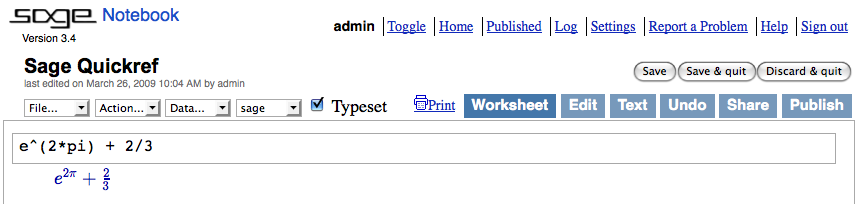
\includegraphics[width=23em]{nb2.png}

Evaluate cell: \shiftEnterkey{}

Evaluate cell creating new cell: \altEnterkey{}

Split cell: \KEYSTROKE{control-;}

Join cells: \controlBackspacekey

Insert math cell: click blue line between cells

Insert text/HTML cell: shift-click blue line between cells

Delete cell: delete content then backspace

%*********************************************
\sect{Command line}

\EXVAR{com}\tabkey{} complete \EXVAR{command}

\EX{*}\EXVAR{bar}\EX{*?} list command names containing ``\sagevar{bar}''

\EXVAR{command}\EX{?}\tabkey{} shows documentation

\EXVAR{command}\EX{??}\tabkey{} shows source code

\EX{a.}\tabkey{} shows methods for object \sagecommand{a} \hfil
(more: \EX{dir(a)})

\EX{a._}\tabkey{} shows hidden methods for object \sagecommand{a} 

\EX{search_doc("}\EXVAR{string or regexp}\EX{")}  fulltext search of docs

\EX{search_src("}\EXVAR{string or regexp}\EX{")}  search source code

\EX{_} is previous output


%*********************************************
\sect{Numbers}

Integers: $\ZZ=$ \EX{ZZ} \@ 
e.g. \EX{-2  -1  0  1  10^100}

Rationals: $\QQ=$ \EX{QQ} \@ 
e.g. \EX{1/2  1/1000  314/100  -2/1}

Reals: $\RR\approx$ \EX{RR} \@ 
e.g. \EX{.5  0.001  3.14  1.23e10000}

Complex: $\CC\approx$ \EX{CC} \@ 
e.g. \EX{CC(1,1)  CC(2.5,-3)}

Double precision: \EX{RDF} and \EX{CDF} \@ 
e.g. 
\EX{CDF(2.1,3)}

Mod $n$: $\ZZ/n\ZZ = $ \EX{Zmod} \@ 
e.g. 
\EX{Mod(2,3)}   
\EX{Zmod(3)(2)}

Finite fields: $\FF_q=$ \EX{GF} \@ 
e.g. 
\EX{GF(3)(2)}   
\EX{GF(9,"a").0}

Polynomials: $R[x,y]$ \@
e.g. 
\EXtt{S.<x,y>=QQ[]}
\EX{x+2*y^3}

Series: $R[[t]]$ \@
e.g. 
\EXtt{S.<t>=QQ[[]]}    
\EX{1/2+2*t+O(t^2)}

$p$-adic numbers: $\ZZ_p\approx$\EX{Zp}, $\mathbf Q_p\approx$\EX{Qp} e.g. \EX{2+3*5+O(5^2)}

Algebraic closure: $\overline{\QQ} = $ \EX{QQbar} e.g. \EX{QQbar(2^(1/5))}

Interval arithmetic: \EX{RIF} e.g. \EX{RIF((1,1.00001))}

Number field: \EXtt{R.<x>=QQ[];} \EXtt{K.<a>=}\EX{NumberField(x^3+x+1)}


%*********************************************
 \sect{Arithmetic}

$ab=$ \EX{a*b}        \quad 
$\frac a b=$ \EX{a/b} \quad 
$a^b=$ \EX{a^b}       \quad 
$\sqrt{x}=$ \EX{sqrt(x)}\\
$\sqrt[n]{x}=$ \EX{x^(1/n)}  \quad 
$|x|=$ \EX{abs(x)}           \quad 
$\log_b(x)=$ \EX{log(x,b)}

Sums:
$\displaystyle
\sum_{i=k}^n f(i)=$ \EX{sum(f(i) for i in (k..n))}

Products:
$\displaystyle
\prod_{i=k}^n f(i)=$ \EX{prod(f(i) for i in (k..n))}


%*********************************************
\sect{Constants and functions}

Constants: 
$\pi=$ \EX{pi} \quad 
$e=$ \EX{e} \quad 
$i=$ \EX{i} \quad 
$\infty=$ \EX{oo} \\
$\phi=$ \EX{golden_ratio} \quad 
$\gamma=$ \EX{euler_gamma}

Approximate: \EX{pi.n(digits=18)} $=3.14159265358979324$

Functions: \EX{sin cos tan sec csc cot sinh cosh tanh sech csch coth log ln exp} \ldots

Python function: \EX{def f(x): return x^2}

%*********************************************
\sect{Interactive functions}

Put \EX{@interact} before function (vars determine controls)
                                                     {\ex\BreakLineAndIndent
\verb|@interact|                                         \BreakLineAndIndent
\verb|def f(n=[0..4], s=(1..5), c=Color("red")):|        \BreakLineAndIndent
\verb|    var("x")|                                      \BreakLineAndIndent
\verb|    show(plot(sin(n+x^s),-pi,pi,color=c))|}

%*********************************************
\sect{Symbolic expressions}

Define new symbolic variables: \EX{var("t u v y z")}

Symbolic function: e.g. $f(x)=x^2$ \@ \EX{f(x)=x^2}

Relations: \EXtt{f==g  f<=g  f>=g  f<g  f>g}

Solve $f=g$: \EX{solve(f(x)==g(x), x)}
\BreakLineAndIndent[\phantom{Solve $f=g$:}]
\EX{solve([f(x,y)==0, g(x,y)==0], x,y)}

\EX{factor(...)}\qquad 
\EX{expand(...)}\qquad 
\EX{(...).simplify_...} 

\EX{find_root(f(x), a, b)} find $x\in [a,b]$ s.t. $f(x)\approx 0$

%*********************************************
\sect{Calculus}

$\displaystyle\lim_{x\to a} f(x)=$ \EX{limit(f(x), x=a)}

$\frac{d}{dx}(f(x))=$ \EX{diff(f(x),x)}                    \\
$\frac{\partial}{\partial x}(f(x,y))=$ \EX{diff(f(x,y),x)} \BreakLineAndIndent
\EX{diff} $=$ \EX{differentiate} $=$ \EX{derivative}

$\int f(x)dx=$ \EX{integral(f(x),x)}                       \\
$\int_a^b f(x)dx=$ \EX{integral(f(x),x,a,b)}               \\
$\int_a^b f(x)dx \approx$ \EX{numerical_integral(f(x),a,b)}

Taylor polynomial, deg $n$ about $a$: \EXtt{taylor(f(x),x,$a$,$n$)}


%*********************************************
\sect{2D graphics}

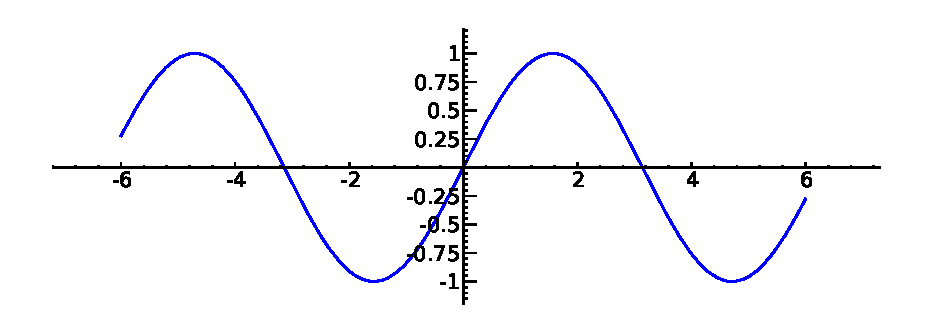
\includegraphics[width=12em]{2d.eps}

\EXtt{line([($x_1$,$y_1$),$\ldots$,($x_n$,$y_n$)],\EXVAR{options})}

\EXtt{polygon([($x_1$,$y_1$),$\ldots$,($x_n$,$y_n$)],\EXVAR{options})}

\EXtt{circle(($x$,$y$),$r$,\EXVAR{options})}

\EXtt{text("txt",($x$,$y$),\EXVAR{options})}

\sagevar{options} as in \sagecommand{plot.options}, \BreakLineAndIndent
e.g. \EX{thickness=}\EXVAR{pixel}, 
\EXtt{rgbcolor=($r$,$g$,$b$)},
\EXtt{hue=$h$}                                      \BreakLineAndIndent
where $0\le r,b,g,h\le 1$

\EXtt{show(\EXVAR{graphic}, \EXVAR{options})}       \BreakLineAndIndent
use \EX{figsize=[w,h]} to adjust size               \BreakLineAndIndent
use \EX{aspect_ratio=}\EXVAR{number} to adjust aspect ratio


\EXtt{plot(f($x$),$(x, x_{\rm min}, x_{\rm max})$,\EXVAR{options})}

\EXtt{parametric\_plot((f($t$),g($t$)),$(t, t_{\rm min}, t_{\rm max})$,\EXVAR{options})}

\EXtt{polar\_plot(f($t$),$(t, t_{\rm min}, t_{\rm max})$,\EXVAR{options})}

combine: \EX{circle((1,1),1)+line([(0,0),(2,2)])}

\EX{animate(}\EXVAR{list of graphics, options}\EX{).show(delay=20)}

%*********************************************
\sect{3D graphics}
 
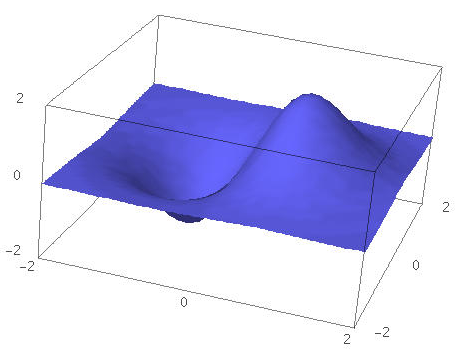
\includegraphics[width=15em,height=8em]{3d.png}

\EXtt{line3d([($x_1$,$y_1$,$z_1$),$\ldots$,($x_n$,$y_n$,$z_n$)],\EXVAR{options})}

\EXtt{sphere(($x$,$y$,$z$),$r$,\EXVAR{options})}

\EXtt{text3d("txt", ($x$,$y$,$z$), \EXVAR{options})}

\EXtt{tetrahedron(($x$,$y$,$z$),$size$,\EXVAR{options})}

\EXtt{cube(($x$,$y$,$z$),$size$,\EXVAR{options})}

\EXtt{octahedron(($x$,$y$,$z$),$size$,\EXVAR{options})}

\EXtt{dodecahedron(($x$,$y$,$z$),$size$,\EXVAR{options})}

\EXtt{icosahedron(($x$,$y$,$z$),$size$,\EXVAR{options})}

\EXtt{plot3d(f($x,y$),$(x,x_{\rm b},x_{\rm e})$, $(y,y_{\rm b},y_{\rm e})$,\EXVAR{options})}

\EXtt{parametric\_plot3d((f,g,h),$(t, t_{\rm b}, t_{\rm e})$,\EXVAR{options})}

\EXtt{parametric\_plot3d((f($u,v$),g($u,v$),h($u,v$)),}
\BreakLineAndFulshLeft
\EXtt{$(u,u_{\rm b},u_{\rm e})$,$(v,v_{\rm b},v_{\rm e})$,\EXVAR{options})}

\sagevar{options}: \EX{aspect_ratio=[1,1,1]}, \EX{color="red"}, 
\BreakLineAndIndent
\EX{opacity=0.5}, \EX{figsize=6}, \EX{viewer="tachyon"}

%*********************************************
\sect{Discrete math}

$\lfloor x\rfloor=$ \EX{floor(x)}
\quad 
$\lceil x\rceil=$ \EX{ceil(x)}

Remainder of $n$ divided by $k=$ {\ex\verb|n%k|}\quad\, 
$k|n$ iff \verb| n%k==0|

$n!=$ \EX{factorial(n)} \qquad
${x\choose m}=$ \EX{binomial(x,m)}

$\phi(n)=$ \EXtt{euler\_phi($n$)}

Strings: e.g. \ \EX{s = "Hello"} = \EX{"He"+'llo'}   \BreakLineAndIndent
\EXtt{s[0]="H" \quad s[-1]="o" \quad s[1:3]="el" \quad s[3:]="lo"}

Lists: e.g. \ \EX{[1,"Hello",x]} = \EX{[]+[1,"Hello"]+[x]}

Tuples: e.g. \ \EX{(1,"Hello",x)} \quad (immutable)

Sets: e.g. \ $\{1,2,1,a\}=$ \EX{Set([1,2,1,"a"])} \ ($=\{1,2,a\}$)

List comprehension $\approx$ set builder notation,
 e.g. \BreakLineAndIndent
$\{f(x)|x\in X, x>0\}=$\EXtt{Set([f(x) for x in X if x>0])}

 
%*********************************************
\sect{Graph theory}

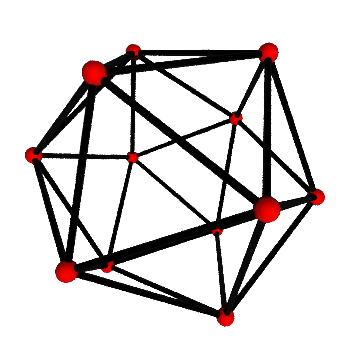
\includegraphics[width=6em]{graph.png}  

Graph: \EXtt{G = Graph(\{0:[1,2,3], 2:[4]\})}

Directed Graph: \EXtt{DiGraph(\EXVAR{dictionary})}

Graph families: \EX{graphs.}\tabkey  

Invariants: \EX{G.chromatic_polynomial()}, \EX{G.is_planar()}

Paths: \EX{G.shortest_path()}

Visualize: \EX{G.plot()}, \EX{G.plot3d()}

Automorphisms: \EX{G.automorphism_group()},
\BreakLineAndIndent
\EX{G1.is_isomorphic(G2)}, \EX{G1.is_subgraph(G2)}


%*********************************************
\sect{Combinatorics}

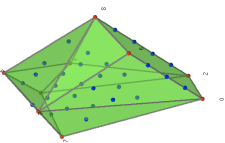
\includegraphics[width=8em]{polytope.png}

Integer sequences: \EXtt{sloane\_find(\EXVAR{list})}, \EXtt{sloane.}\tabkey  

Partitions:
\EXtt{P=Partitions(\EXvar{n})}\quad \EX{P.count()}

Combinations: \EXtt{C=Combinations(\EXVAR{list})}\quad\EX{C.list()}

Cartesian product: \EX{CartesianProduct(P,C)}

Tableau: \EX{Tableau([[1,2,3],[4,5]])}

Words: \EX{W=Words("abc"); W("aabca")}

Posets: \EX{Poset([[1,2],[4],[3],[4],[]])}

Root systems: \EX{RootSystem(["A",3])}

Crystals: \EX{CrystalOfTableaux(["A",3], shape=[3,2])}

Lattice Polytopes: \EX{A=random_matrix(ZZ,3,6,x=7)}\\
\EX{L=LatticePolytope(A)    L.npoints()   L.plot3d()}

%*********************************************
\sect{Matrix algebra}

$\begin{pmatrix}1\\2\end{pmatrix}=$ 
\EX{vector([1,2])}

$\begin{pmatrix}1&2\\3&4\end{pmatrix}=$ 
\EX{matrix(QQ,[[1,2],[3,4]], sparse=False)}

$\begin{pmatrix}1&2&3\\4&5&6\end{pmatrix}=$ 
\EX{matrix(QQ,2,3,[1,2,3, 4,5,6])}

$\left|\begin{matrix}1&2\\3&4\end{matrix}\right|=$
\EX{det(matrix(QQ,[[1,2],[3,4]]))}

$Av=$ \EX{A*v} \quad $A^{-1}=$ \EX{A^-1} \quad $A^t=$ \EX{A.transpose()}

Solve $Ax=v$: \EX{A\v} or \EX{A.solve_right(v)}

Solve $xA=v$: \EX{A.solve_left(v)}

Reduced row echelon form: \EX{A.echelon_form()}

Rank and nullity: \EX{A.rank()    A.nullity()}

Hessenberg form: \EX{A.hessenberg_form()}

Characteristic polynomial: \EX{A.charpoly()}

Eigenvalues: \EX{A.eigenvalues()}

Eigenvectors: \EX{A.eigenvectors_right()} (also left)

Gram-Schmidt: \EX{A.gram_schmidt()}

Visualize: \EX{A.plot()}

LLL reduction: \EX{matrix(ZZ,...).LLL()}

Hermite form: \EX{matrix(ZZ,...).hermite_form()}

%*********************************************
\sect{Linear algebra}

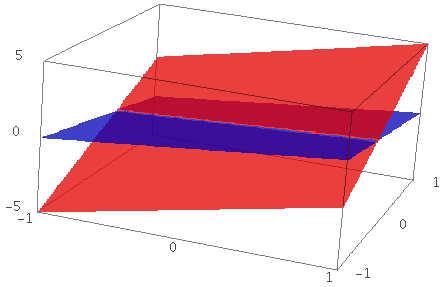
\includegraphics[width=12em,height=6em]{linalg.png}

Vector space $K^n = $ \EX{K^n} e.g. \EX{QQ^3   RR^2   CC^4}

Subspace: \EX{span(vectors, }\EXVAR{field}\EX{)}
\BreakLineAndIndent
E.g., \EX{span([[1,2,3], [2,3,5]], QQ)}

Kernel: \EX{A.right_kernel()} (also left)

Sum and intersection: \EX{V + W} and \EX{V.intersection(W)}

Basis: \EX{V.basis()}

Basis matrix: \EX{V.basis_matrix()}

Restrict matrix to subspace: \EX{A.restrict(V)}

Vector in terms of basis: \EXtt{V.coordinates(\EXVAR{vector})}

%*********************************************
\sect{Numerical mathematics}

Packages: \EX{import numpy, scipy, cvxopt}

Minimization: \EX{var("x y z")}
\BreakLineAndIndent
\EX{minimize(x^2+x*y^3+(1-z)^2-1, [1,1,1])}


%*********************************************
\sect{Number theory}

Primes: \EX{prime_range(n,m)}, \EX{is_prime}, \EX{next_prime}

Factor: \EX{factor(n)}, \EX{qsieve(n)}, \EX{ecm.factor(n)}

Kronecker symbol: $\left(\frac{a}{b}\right) = $ \EXtt{kronecker\_symbol(\EXvar{a},\EXvar{b})}

Continued fractions: \EX{continued_fraction(x)}

Bernoulli numbers: \EX{bernoulli(n)}, \EX{bernoulli_mod_p(p)}

Elliptic curves: \EXtt{EllipticCurve([$a_1,a_2,a_3,a_4,a_6$])}

Dirichlet characters: \EXtt{DirichletGroup(\EXvar{N})}

%Congruence subgroups: \texttt{Gamma0({\it N})}, \texttt{Gamma1({\it N})}, \texttt{GammaH}

Modular forms: \EXtt{ModularForms(\EXVAR{level}, \EXVAR{weight})}

Modular symbols: \EXtt{ModularSymbols(\EXVAR{level},\EXVAR{weight},\EXVAR{sign})}

Brandt modules: \EXtt{BrandtModule(\EXVAR{level}, \EXVAR{weight})}

Modular abelian varieties: \EXtt{J0(\EXvar{N})}, \EXtt{J1(\EXvar{N})}

%*********************************************
\sect{Group theory}

\EX{G = PermutationGroup([[(1,2,3),(4,5)],[(3,4)]])}

\EXtt{SymmetricGroup(\EXvar{n})}, \EXtt{AlternatingGroup(\EXvar{n})} 

Abelian groups: \EX{AbelianGroup([3,15])}

Matrix groups: \EX{GL}, \EX{SL}, \EX{Sp}, \EX{SU}, \EX{GU}, \EX{SO}, \EX{GO}

Functions: \EX{G.sylow_subgroup(p)}, \EX{G.character_table()}, 
\BreakLineAndIndent
\EX{G.normal_subgroups()}, \EX{G.cayley_graph()}


%*********************************************
\sect{Noncommutative rings}

Quaternions: \EXtt{Q.<i,j,k> = QuaternionAlgebra(a,b)}

Free algebra: \EXtt{R.<a,b,c> = FreeAlgebra(QQ, 3)}

%Steenrod algebra: \texttt{SteenrodAlgebra({\it prime})}

%*********************************************
\sect{Python modules}

\EX{import} \EXVAR{module_name}

\EX{module_name.}\tabkey{} and \EX{help(module_name)}

%\verb|sage.|\emph{module\_name}\verb|.all.|$\langle$tab$\rangle$ shows exported commands

%\mbox{Std packages: Maxima GP/PARI GAP Singular R Shell ...}

%Opt packages: Biopython Gnuplot Kash ...

%\%\emph{package\_name} then use package command syntax

%*********************************************
\sect{Profiling and debugging}

\EX{time} \EXVAR{command}:   show timing information    \\
\EX{timeit("command")}: accurately time command

\EX{t = cputime(); cputime(t)}: elapsed CPU time       \\
\EX{t = walltime(); walltime(t)}: elapsed wall time

{\ex\verb|%pdb|}: turn on interactive debugger (command line only) \\
{\ex\verb|%prun command|}: profile command (command line only)

\end{multicols*}

\end{document}
